\newcommand{\figO}{
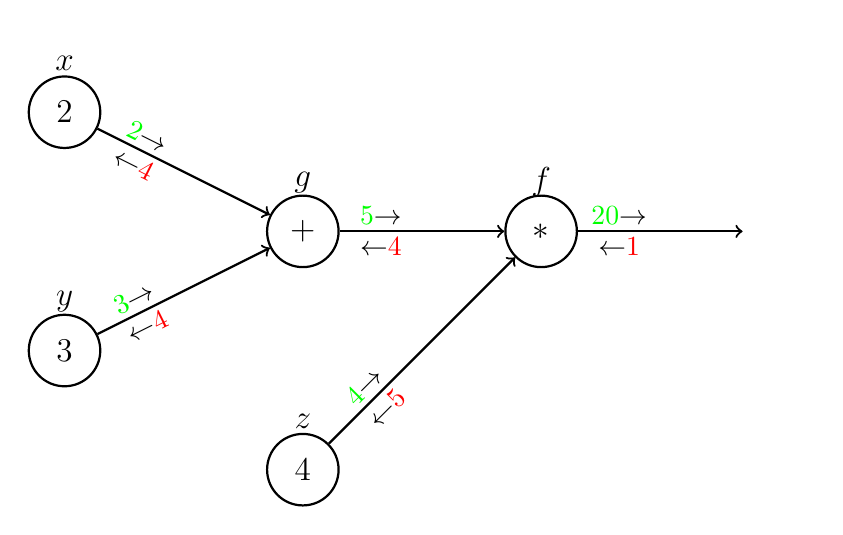
\begin{tikzpicture}[x = 10ex, y= 10ex,
        every node/.style={circle,draw, minimum size = 6ex, font=\large},
        every path/.style={->, thick}
]
    \node[label={[label distance=-9pt]90:$x$}] (x) at (1,-1) {$2$};
    \node[label={[label distance=-9pt]90:$y$}] (y) at (1,-3) {$3$};
    \node[label={[label distance=-9pt]90:$g$}] (g) at (3,-2) {$+$};
    \node[label={[label distance=-9pt]90:$z$}] (z) at (3,-4) {$4$};
    \node[label={[label distance=-9pt]90:$f$}] (f) at (5,-2) {$*$};
    \node[draw=none] (loss) at (7,-2) {};
\begin{scope}[every node/.style={inner sep=1pt}]
    \draw (x) -- node [near start, above=1pt, sloped] {\textcolor{green}{2}$\rightarrow$} node [near start, below=1pt, sloped] {$\leftarrow$\textcolor{red}{4}} (g);
    \draw (y) -- node [near start, above=1pt, sloped] {\textcolor{green}{3}$\rightarrow$} node [near start, below=1pt, sloped] {$\leftarrow$\textcolor{red}{4}} (g);
    \draw (g) -- node [near start, above=1pt, sloped] {\textcolor{green}{5}$\rightarrow$} node [near start, below=1pt, sloped] {$\leftarrow$\textcolor{red}{4}} (f);
    \draw (z) -- node [near start, above=1pt, sloped] {\textcolor{green}{4}$\rightarrow$} node [near start, below=1pt, sloped] {$\leftarrow$\textcolor{red}{5}} (f);
    \draw (f) -- node [near start, above=1pt, sloped] {\textcolor{green}{20}$\rightarrow$} node [near start, below=1pt, sloped] {$\leftarrow$\textcolor{red}{1}} (loss);
\end{scope}

\end{tikzpicture}
}
\newcommand{\figT}{
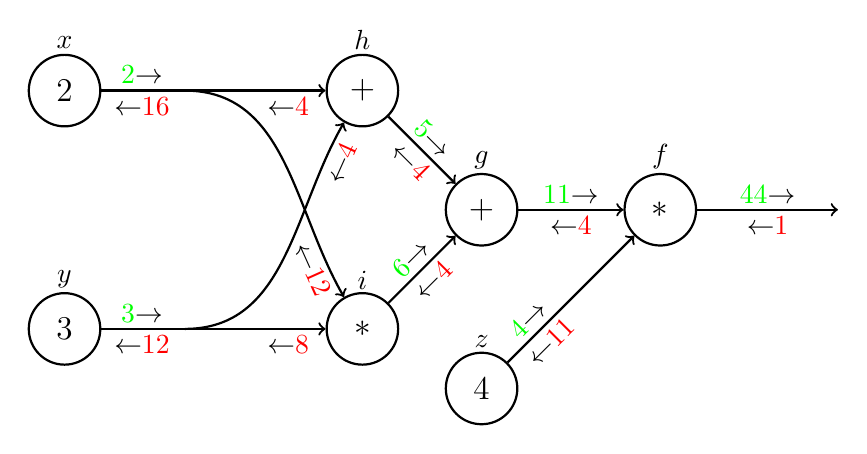
\begin{tikzpicture}[x = 10ex, y= 10ex,
        every node/.style={inner sep=0pt, minimum size = -2ex, shape=circle},
        every path/.style={->, thick}
]
\tikzstyle{block}= [draw, circle, minimum size = 6ex, font=\large]
    \node[block, label={[label distance=0pt]90:$x$}] (x) at (1.5,-1) {$2$};
    \node[block, label={[label distance=0pt]90:$y$}] (y) at (1.5,-3) {$3$};
    \node (dx) at (2.5, -1) {};
    \node (dy) at (2.5, -3) {};
    \node[block, label={[label distance=0pt]90:$h$}] (h) at (4,-1) {$+$};
    \node[block, label={[label distance=0pt]90:$i$}] (i) at (4,-3) {$*$};
    \node[block, label={[label distance=0pt]90:$g$}] (g) at (5,-2) {$+$};
    \node[block, label={[label distance=0pt]90:$z$}] (z) at (5,-3.5) {$4$};
    \node[block, label={[label distance=0pt]90:$f$}] (f) at (6.5,-2) {$*$};
    \node[draw=none] (loss) at (8,-2) {};
\begin{scope}[every node/.style={inner sep=1pt}]

    \draw[-,shorten >=-1pt] (x) -- node [midway, above=1pt, sloped] {\textcolor{green}{2}$\rightarrow$} node [midway, below=1pt, sloped] {$\leftarrow$\textcolor{red}{16}} (dx);
    \draw (dx) to [out=0,in=180,swap] node [near end, below=1pt, sloped] {$\leftarrow$\textcolor{red}{4}} (h);
    \draw (dx) to [out=0,in=120,swap] node [very near end, below=1pt, sloped] {$\leftarrow$\textcolor{red}{12}} (i);
    \draw[-,shorten >=-1pt] (y) -- node [midway, above=1pt, sloped] {\textcolor{green}{3}$\rightarrow$} node [midway, below=1pt, sloped] {$\leftarrow$\textcolor{red}{12}} (dy);
    \draw (dy) to [out=0,in=180,swap] node [near end, below=1pt, sloped] {$\leftarrow$\textcolor{red}{8}} (i);
    \draw (dy) to [out=0,in=240,swap] node [very near end, below=1pt, sloped] {$\leftarrow$\textcolor{red}{4}} (h);
    \draw (h) to node [midway, above=1pt, sloped] {\textcolor{green}{5}$\rightarrow$} node [midway, below=1pt, sloped] {$\leftarrow$\textcolor{red}{4}} (g);
    \draw (i) to node [midway, above=1pt, sloped] {\textcolor{green}{6}$\rightarrow$} node [midway, below=1pt, sloped] {$\leftarrow$\textcolor{red}{4}} (g);
    \draw (g) to node [midway, above=1pt, sloped] {\textcolor{green}{11}$\rightarrow$} node [midway, below=1pt, sloped] {$\leftarrow$\textcolor{red}{4}} (f);
    \draw (z) -- node [near start, above=1pt, sloped] {\textcolor{green}{4}$\rightarrow$} node [near start, below=1pt, sloped] {$\leftarrow$\textcolor{red}{11}} (f);
    \draw (f) -- node [midway, above=1pt, sloped] {\textcolor{green}{44}$\rightarrow$} node [midway, below=1pt, sloped] {$\leftarrow$\textcolor{red}{1}} (loss);
\end{scope}

\end{tikzpicture}
}


\newcommand{\figTh}{
\begin{tikzpicture}[x = 10ex, y= 10ex,
        every node/.style={inner sep=0pt, minimum size = -2ex, shape=circle},
        every path/.style={->, thick}
]
\tikzstyle{matrix}= [draw, circle, minimum size = 7ex, font=\large]
\tikzstyle{func}= [draw, circle, minimum size = 4ex, font=\large]
    \node[matrix] (A11) at (1,-2) {$A_{1, 1}$};
    \node (int1) at (1, -3) {};
    \node[matrix] (A12) at (3,-2) {$A_{1, 2}$};
    \node (int2) at (3, -3) {};
    \node[func] (a1x) at (1.5,-5) {$*$};
    \node[func] (a2x) at (2.5, -5) {$*$};
    \node[func] (axx) at (2, -6) {$+$};
    \node[matrix] (B11) at (6,-1) {$B_{1, 1}$};
    \node[matrix] (B12) at (8, -1) {$B_{1, 2}$};
    \node[matrix] (B21) at (6, -3) {$B_{2, 1}$};
    \node[matrix] (B22) at (8, -3) {$B_{2, 2}$};
    \node[func] (b1x) at (5.75, -5) {$*$};
    \node[func] (b2x) at (6.75, -5) {$*$};
    \node[func] (bxx) at (6.25, -6) {$+$};
    \node[draw=none] (f1) at (2,-7) {};
    \node[draw=none] (f2) at (6.25, -7) {};
\begin{scope}[every node/.style={inner sep=1pt}]

    \draw[-,shorten >=-1pt] (A11) -- (int1);
    \draw (int1) to [out=270,in=90,swap] (a1x);
    \draw (int1) to [out=270,in=120,swap] (b1x);
    \draw[-,shorten >=-1pt] (A12) -- (int2);
    \draw (int2) to [out=270,in=90,swap] (a2x);
    \draw (int2) to [out=270,in=100,swap] (b2x);
    \draw (B11) to (a1x);
    \draw (B21) to (a2x);
    \draw (B12) to (b1x);
    \draw (B22) -- (b2x);
    \draw (a1x) -- (axx);
    \draw (a2x) -- (axx);
    \draw (b1x) -- (bxx);
    \draw (b2x) -- (bxx);
    \draw (axx) -- (f1);
    \draw (bxx) -- (f2);
    \node [shape=rectangle, rounded corners=10pt, draw=black, fit= (A11) (A12), inner sep=0.75cm] {\Large$\boldsymbol{A}$};
    \node [shape=rectangle, rounded corners=10pt, draw=black, fit= (B11) (B12) (B21) (B22), inner sep=0.75cm] {\Large$\boldsymbol{B}$};
    \node [shape=rectangle, rounded corners=10pt, draw=black, fit= (a1x) (a2x) (b1x) (b2x) (axx) (bxx), inner sep=0.75cm] {\Large$\boldsymbol{f}$};
\end{scope}

\end{tikzpicture}
}

\newcommand{\figTi}{
\begin{tikzpicture}[x = 10ex, y= 10ex,
        every node/.style={circle,draw, minimum size = 6ex, font=\large},
        every path/.style={->, thick}
]
    \node[label={[label distance=-9pt]90:$x$}] (x) at (1,-1) {$2$};
    \node[label={[label distance=-9pt]90:$y$}] (y) at (1,-3) {$3$};
    \node[label={[label distance=-9pt]90:$g$}] (g) at (3,-2) {$+$};
    \node[label={[label distance=-9pt]90:$z$}] (z) at (3,-4) {$4$};
    \node[label={[label distance=-9pt]90:$f$}] (f) at (5,-2) {$*$};
    \node[draw=none] (loss) at (7,-2) {};
\begin{scope}[every node/.style={inner sep=1pt}]
    \draw (x) -- node [near start, above=1pt, sloped] {} node [near start, below=1pt, sloped] {} (g);
    \draw (y) -- node [near start, above=1pt, sloped] {} node [near start, below=1pt, sloped] {} (g);
    \draw (g) -- node [near start, above=1pt, sloped] {} node [near start, below=1pt, sloped] {} (f);
    \draw (z) -- node [near start, above=1pt, sloped] {} node [near start, below=1pt, sloped] {} (f);
    \draw (f) -- node [near start, above=1pt, sloped] {} node [near start, below=1pt, sloped] {} (loss);
\end{scope}

\end{tikzpicture}
}